\chapter{The Survey: Captures, Trawl, \& Products}
\label{sec:survey}

The survey is the bridge between a verified detector and a scientific claim.
It applies the detector to archival telescope data, preserves enough intermediate
information to revisit the decision later, and records where the archive cannot
support an inference.  This chapter therefore distinguishes three objects that
are easy to conflate: the \emph{available archive}, the \emph{processing
inventory}, and the \emph{population of telescope time} about which one might
want to make a statement.  The first two are measurable from logs.  The third
requires a selection model, because the archive consists of triggered snapshots
rather than a uniform observing stream.

\begin{figure}[t]
\centering
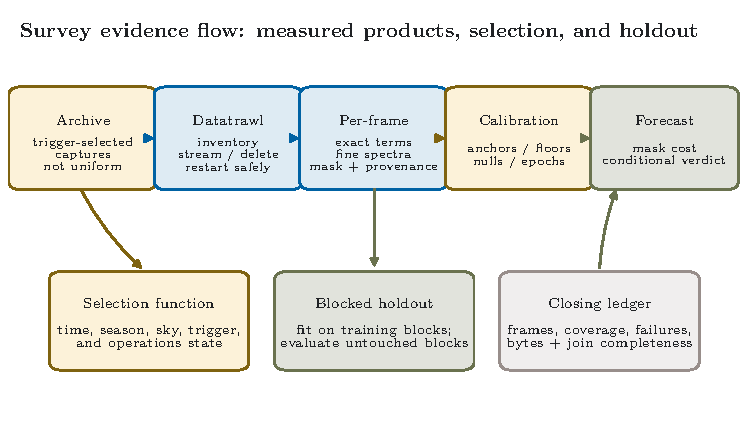
\includegraphics[width=0.98\linewidth]{figs/fig_survey_evidence_flow.pdf}
\caption[Survey evidence flow and claim boundary]{The survey evidence flow.
Triggered baseband captures are inventoried before processing; the restartable
trawl produces exact detector terms, fine spectra, decisions, and provenance;
calibration and forecast products are derived from those records.  The dashed
boundary is load-bearing: a triggered archive is not automatically a random
sample of transmitter occupancy.  Selection diagnostics and blocked holdout
validation are therefore part of the scientific product, not optional metadata.}
\label{fig:survey:evidenceflow}
\end{figure}

\section{Triggered Baseband Captures and Their Selection Function}
\label{sec:survey:data}

The raw material is the archive of full-array baseband captures recorded by the
telescope's transient backend \cite{amiri2018frb}.  A capture contains the packed
$4{+}4$-bit channelized stream for all $M=2048$ inputs and spans seconds rather
than a continuous day.  The trawl completed in August 2026, and the archive now
carries products for all 23 ATSC allocations (channels 14--36), each complete
against its archive holdings:
the survey enumerates $16{,}327$ events, excludes $6{,}140$ carrying the
recorded outrigger label, and therefore targets $10{,}187$ events.  Of those,
$10{,}184$ have completed dispositions, while three are frozen in the source
inventory's pending-attempt category after two recorded attempts; their three
unprocessed units are the released quarantines, not an active retry queue.  The completed partition contains
$9{,}214$ distinct events represented by inventory rows, $107$ aged-out empty
events, and $863$ events derived by set subtraction as lacking a common target
path; the individual status ledger for that last category did not survive.  The inventory has
$170{,}377$ unique event--channel source objects, of which $170{,}374$ are
processed product units and the remaining three are exactly the three
quarantines; the release itself contains 23 per-channel NPZ products and
$750{,}461$ stored
detector frames.  Of these frames, $750{,}457$ satisfy the analyzer's original
denominator-validity rule and four all-zero frames are explicitly invalid.  A
versioned post-processing health gate, described below, retains $750{,}279$
frames from $8{,}980$ distinct events for scientific summaries, compared with
$8{,}983$ events having at least one stored denominator-valid frame.  The wider
product inventory includes $4{,}692$ event--channel units shorter than one
complete $N=16384$ frame; retaining those zero-frame units in the ledger is
important because ``discovered and readable'' is not the same denominator as
``contributed a detector frame.''  The stored-frame population has a
median of three $N=16384$ detector frames per
acquisition; calendar coverage from December 2018 through July 2026; three
raw objects quarantined before unit construction (two truncated, one with an unreadable
header); and one detector-kernel binary, represented by two analyzer
source-build cohorts,
across every product.  Per-channel event counts are far from uniform ---
$1{,}543$ to $9{,}045$ --- and the deficit is concentrated on exactly the two
most contaminated channels, for the selection reason discussed below.  Those
figures describe the working archive at snapshot time; the immutable release
ledger, rather than this prose, is the authoritative denominator.

A post-completion input-health audit exposed a second validity layer that the
archived denominator rule did not test.  In 178 rows from eight source events,
the recorded mean baseband power is exactly $128$, the maximum possible value
of $x_r^2+x_i^2$ after the native excess-8 complex \texttt{int4} samples are
decoded to $[-8,7]$.  Equality of a frame-wide mean at that upper bound is
possible only when every decoded sample is $(-8,-8)$: native raw byte
\texttt{0x00}, equivalently detector-input byte \texttt{0x88} after the ingest
adapter's lossless XOR-\texttt{0x88} repack.  This establishes a constant
ceiling word rather than ordinary receiver noise.  It does not identify why the
acquisition path produced that word, but the cause is no longer needed to make
the scientific validity decision: a constant negative-full-scale frame is not
a measurement of receiver noise or sky voltage.  The released
\texttt{pilotproxy\_archive\_frame\_health\_gate\_v1} therefore excludes all
178 rows with reason code
\texttt{baseband\_power\_at\_negative\_full\_scale\_ceiling}, as well as the
four already-invalid all-zero rows.  These reason sets do not overlap, so the
gate removes 182 unique rows and retains $750{,}279$.

The absence of per-frame voltage spectra would normally prevent an exact
retrospective spectral repair.  Here the excluded valid frames are a special,
fully determined case: a constant frame contributes only to the unshifted FFT
bin zero.  Reproducing the analyzer's actual complex64 absolute-square followed
by float64 stream sum gives a contribution of
$70{,}368{,}739{,}983{,}360$ per frame at that bin and exactly zero elsewhere.
The repair subtracts this amount for all 178 rows from the before-mask
accumulator and for the 118 rows that the stored coarse rule had kept from the
after-mask accumulator; the other 60 had already been rejected.  Every repaired
spectrum remains non-negative and passes an independent Parseval comparison to
the health-included frame-power sum within the declared $5\times10^{-7}$
relative tolerance.  This exceptional reconstruction does not create general
per-frame voltage spectra: arbitrary remasking would still require the source
HDF5 files.

The input attachments, gate identity, affected physical keys, exact spectral
correction, and reason-coded disposition are frozen in
\verb|CANFAR_PRODUCT_HEALTH_AUDIT.json| and the PilotProxy exclusion ledger.
Retrieving raw HDF5 data could still diagnose the acquisition-side cause, but
it is now an optional engineering investigation rather than a blocker on the
health-filtered scientific estimand.

Appendix~\ref{app:archive-diagnostics} exposes the regenerated evidence rather
than reducing it to one headline count.  For each of the 23 physical channels
it provides health-filtered histograms of the coarse statistic, normalized
coarse level, decoded input power, and a fine ratio whose window is either a
narrow measured quarterly anchor or an explicit broad predicted-neighbourhood
fallback;
an exactly health-corrected relative time-averaged before/after spectrum; and a
UTC-monthly fine-statistic waterfall.  The last object is the most informative
time--frequency view supported by the saved products, but it is not called a
raw spectrogram: the products retain the full fine-$F$ vector per detector
frame and only two accumulated voltage-spectrum powers.  This distinction
prevents a visually useful diagnostic from implying frequency resolution,
absolute calibration, or post-hoc remasking that the archive cannot supply.
The broad predicted neighbourhood repairs the obsolete bin-zero diagnostic,
while the measured/refused quarterly records expose what the retained array can
support without pretending that this retrospective partition is a prospective
holdout.  Both are kept distinct from the authoritative station-epoch anchor,
exact Q16 threshold, and blocked validation needed for a final decision bundle.

The captures were not selected by the DTV detector.  They were initiated by the
transient system and filtered by telescope operations, data availability,
archive retention, and later inventory rules.  One of those filters is now
measured and deserves emphasis because it is \emph{endogenous to the
contamination itself}: the telescope curtails baseband collection on its most
contaminated coarse channels, and captures on the channel-30 monitored bin
cease entirely after September 2023 --- an operations exclusion driven by the
DTV occupancy this survey measures.  Archive completeness is therefore
correlated with the quantity under study; the thin channel-30 and channel-24
inventories are a selection effect, not a property of the transmitters, and a
channel excluded from collection can never report a subsequent transmitter
sign-off from this archive (five sign-offs or station departures were recorded on collected channels
during the survey span, so the possibility is not hypothetical).  Let $I(t,c)$
be the indicator that telescope time $t$ on channel $c$ enters the survey.  The occupancy quantity
measured directly by the survey is
\begin{equation}
  \Pr(\text{DTV state}\mid I=1,c),
\end{equation}
not the unconditional time occupancy $\Pr(\text{DTV state}\mid c)$ unless the
inclusion process is ignorable for the variables controlling propagation and
transmitter state.  Time of day, season, sidereal time, weather, trigger class,
commissioning state, and station-era boundaries are all plausible dependencies.
The archive can still support a strong detector and calibration study, but its
masked fractions are explicitly \emph{archive fractions} until the selection
comparison is completed.

\begin{table}[t]
\centering
\caption{Survey inventory fields after reconciliation of the products,
inventory attachment, quarantine ledger, and v1 health ledger.  ``Not
recorded'' is an evidence state, not a numerical zero, and catalogued bytes are
not relabelled as transferred bytes.}
\label{tab:survey:inventory}
\begin{tabularx}{\linewidth}{>{\raggedright\arraybackslash}p{0.30\linewidth}
                             >{\raggedright\arraybackslash}p{0.22\linewidth}
                             >{\raggedright\arraybackslash}X}
\toprule
Inventory field & Recorded value/status & Provenance or remaining limitation \\
\midrule
Calendar coverage & Dec 2018--Jul 2026 & Per-channel first/last stored and health-included UTC released; calendar-month gaps are preserved in Appendix~\ref{app:archive-diagnostics} \\
Capture events per analyzed channel & $1{,}543$--$9{,}045$ ($9{,}214$ distinct inventory-represented events; all 23 allocations) & $170{,}377$ unique inventory objects $=170{,}374$ processed event--channel units $+3$ quarantines; 23 per-channel NPZ products; no duplicate inventory keys \\
Frames per acquisition & median 3; $750{,}461$ stored; $750{,}279$ v1-health-included; 182 reason-coded exclusions & Full distribution and immutable frame-level exclusion ledger released \\
Longest contiguous statistic used here & 1.38~s & Per-unit frame counts and 4,692 zero-frame units retained; the source logs do not preserve every acquisition-side truncation reason \\
Raw and derived storage & $28{,}237{,}618{,}443{,}352$ catalogued source bytes & This is discovered object size, not measured transfer volume; transfer, cache, deletion, and peak-stage telemetry were not retained \\
Retry attempts & 3 scope events have two recorded attempts & The inventory preserves the attempt multiplicity, but not a reason code or per-attempt resource measurements; the three second attempts are the only recorded retries \\
Trawl throughput and wall time & not recorded & Frames/s, transferred data rate, GPU time, peak staging storage, and end-to-end wall time cannot be reconstructed from the supplied products \\
Selection diagnostics & frame UTC and inventory trigger/scheduled labels retained; operations state incomplete & UTC supports reproducible local-time/season/sidereal projections; no absent operations annotation is inferred \\
\bottomrule
\end{tabularx}
\end{table}

The exposure profiles keep a second denominator because a stored frame is not
automatically a timed frame.  Of the $750{,}279$ health-included frames,
$747{,}790$ have both a finite timestamp and a positive finite frame duration;
the other $2{,}489$ remain in count-based summaries but contribute no invented
seconds to an exposure histogram.  Joining all frame rows back to the supplied
inventory gives $699{,}579$ health-included triggered frames in $166{,}581$
event--channel units and $50{,}700$ scheduled frames in $3{,}793$ units; their
timed subsets contribute $29{,}238.074$~s and $2{,}126.512$~s, respectively.
The release tabulates frame counts and
durations by UTC month and hour, America/Vancouver civil month, hour, and
meteorological season, and local mean sidereal hour.  The last coordinate uses
the declared DRAO longitude ($-119.6175^\circ$) and UTC as a documented proxy
for UT1; it is therefore a reproducible coverage diagnostic, not an
astrometry-grade apparent-sidereal timestamp.  Trigger and scheduled labels are
measured inventory fields.  Operations states that were never recorded remain
unavailable rather than being inferred from those labels.

Two consequences recur later.  First, the snapshot duration caps any contiguous
block statistic that can be reproduced from this archive.  Second, the sparse
spacing leaves a correlation-time blind interval between the frame duration and
typical acquisition separation.  Chapter~\ref{sec:calibration} therefore allows
the correlation estimator to return a measurement, a bound, or a refusal rather
than interpolating across that gap.

\section{A Restartable, Bounded-Storage Trawl}
\label{sec:survey:trawl}

The trawl processes every eligible capture through the same detector arithmetic
described in Chapters~\ref{sec:pipeline} and~\ref{sec:impl}.  It is organized in
three nested units: an inventory entry identifies an archived acquisition, a
processing unit identifies a contiguous readable segment, and a detector frame
is the $N$-sample decision quantum.  This separation allows the operational
machinery to restart without changing the scientific definition of a frame.

The processing environment cannot stage the entire archive locally.  The trawl
therefore follows a bounded-storage cycle: discover an eligible source, pull one
unit, validate it, process all complete frames, write a content-addressed product,
verify the product, and remove the staged source only after the write is durable.
A unit that fails validation is quarantined with its exception and provenance;
it is not silently omitted or counted as a quiet frame.  Resume logic treats an
already verified product as complete only when the source identity, detector
geometry, weight and transform hashes, schema, and science-relevant configuration
match.  A source-code change that leaves those immutable tokens unchanged can be
recorded without forcing a scientifically identical re-run; a kernel, geometry,
or schema change creates a new cohort.

The trawl architecture is intentionally detector-agnostic at the operational
layer.  Inventory, transfer, retry, checkpoint, quarantine, and deletion belong
to the data-management system; the pilot proxy enters through an analyzer
interface that consumes a frame and emits a declared product schema.  This
boundary is why failures in archive access do not become hidden branches in the
signal-processing code, and why the same operational core can support other
large telescope reductions.

\section{Products: Statistics, Not Only Verdicts}
\label{sec:survey:products}

Each product using schema \texttt{pilotproxy\_detector\_datatrawl\_v3} retains,
per frame, the exact target and reference power terms; floating diagnostics such
as the coarse ratio and inferred shelf level; validity and rejection fields; the
complete 256-bin fine statistic; diagnostic CFAR location and scale fields; and
any-bin detection locations.  Product-wide metadata retain the source identity,
weight-bank and transform hashes, resolved reference placement, exact integer
norms, detector and schema versions, and the within-channel spectra used for the
broadcast characterization.

This choice makes the \emph{coarse} threshold exactly reversible.  A product
that stored only a mask bit could answer what one historical policy rejected;
the retained coarse integer terms instead permit any later coarse threshold to
be re-evaluated by the same exact cross-product.  The retained floating-point
fine spectrum likewise supports designated-window, bulk, rank, and threshold
diagnostics and an offline prototype of a later per-epoch policy.  It does not,
however, retain the three unsigned-integer fine powers from which an exact Q16
decision is made.  A threshold-near exact replay of a new fine policy therefore
requires those absent accumulators or a raw-data rerun.  This boundary keeps
implementation verification separate from policy without implying that a
floating diagnostic is an exact substitute for the decision operands.

\section{Reproduction and the Required Denominator}
\label{sec:survey:reproduction}

The supplied products contain two recorded source cohorts: a modern cohort
covering 21 channels and a legacy cohort covering channels 35--36.  They share
the supplied kernel digest, detector geometry, and product schema, but they do
not overlap in channel--event units.  The source history reproduces the modern
cohort's recorded source hash exactly; it does not reproduce the legacy hash.
Consequently this release can verify each product against its contract and
binary provenance, but it cannot verify the older development-note statement
that two independent builds produced ``zero mismatches'' on overlapping
records.  No joined comparison manifest or denominator was supplied, and this
dissertation does not convert that absence into a measured result.

A future cross-build reproduction claim must include

\begin{itemize}[leftmargin=2em]
  \item the number of discovered, eligible, and successfully joined events and frames;
  \item join completeness and the treatment of duplicates, missing products, and invalid frames;
  \item the exact fields and byte representations compared; and
  \item the source, binary, toolkit, weight, transform, schema, and cohort hashes.
\end{itemize}

The versioned health release supplies those denominators for its own product
accounting, validity exclusions, spectrum correction, and regenerated
diagnostics.  It does not retroactively create the absent cross-build join.
Appendix~\ref{app:evidence} therefore records archive-scale accounting as
measured and the historical cross-build comparison as unavailable unless its
independent ledger is recovered.

\section{Selection-Aware Calibration and Holdout Design}
\label{sec:survey:holdout}

Randomly splitting individual frames would overstate independence: neighboring
frames within a capture share receiver state, transmitter state, and propagation,
and frames across a station era can share a persistent offset.  Calibration and
evaluation are therefore blocked at the acquisition or sidereal-day level and
stratified by measured station epoch.  Within each epoch, one block set localizes
anchors and selects $(\rho,\eta)$; disjoint blocks estimate false alarms, masked
fraction, residual levels, and cost.  A stricter leave-one-year-or-era-out check
asks whether the selected operating point transports across calendar structure.

The holdout design cannot make the archive uniform, but it prevents a second,
avoidable optimism: evaluating a threshold on the same correlated frames that
selected it.  The final campaign reports both the within-archive blocked result
and the coverage diagnostics of Table~\ref{tab:survey:inventory}.  Only then can
an archive fraction be promoted to an estimate of observing-time occupancy, and
only over the population for which the coverage comparison supports that move.
